\chapter{System Design}

\section{Business case}

ChatX is a chatting system which will allow users to communicate with each other from where ever they are and without fear of the messages being read by unwanted users, as long as they use a platform that supports the application and have a Internet connection.

\subsection{FURPS}
FURPS is a architectural checklist. It helps describe what areas needs to be focused on, and an overall view of what ChatX's purpose is.

\subsubsection{Functionality}
Functionality deals with requirements the customer has set for the project. To help the customer determine the requirements, a question to ask is: What problem is the system going to solve? And with ChatX, users that are in need of communication with other users from a long distance on a secure connection, making sure that messages are private, and only seen by the intended users.
%making it difficult for third party listeners to sniff data from. Making sure that messages are private, and only seen by the intended users.

\subsubsection{Usability}
Usability describes how accessible ChatX is for the users. Is it easy to use? Is the GUI design intuitive? A way to check if the users like the aesthetics (and more importantly, can see how to use it) would be to prepare usability tests and alpha/beta tests as they can give crucial feedback on how user friendly a system is.

\subsubsection{Reliability} 
Reliability describes how reliable the system should be: How much downtime can it handle? Are failures predictable? How is the system going to recover in case of failure? 

Due to ChatX's architecture it is possible to setup several servers at once and if one fails, then the other servers can be used instead. In worst case scenario if all servers go down, then it would not take too long to install the server software on a different one and ChatX would continue working.

\subsubsection{Performance}Performance describes how fast an application must be, what the highest allowed response time is and how much memory is needed. 

ChatX is a chatting system, meaning that messages has to be sent and received as quickly as possible, however we can only assure a fast reliable service at the server end with optimal coding.
%however it is impossible to assure that since it is unknown how good internet connections the users have.

\subsubsection{Supportability}
Supportability, the last of the FURPS principles, describes how maintainable an application is after it is deployment. It also describes how easy it is to install and configure. 

For ChatX two installations are required, the "server" installation has to be put up on a server, and a client has to install the java "client" on their computers. ChatX has been developed with expansion in mind, as earlier mentioned in case of server side errors, another one can easily take its place. The same principle applies here, if for whatever a reason someone chooses to shut down the server, it would be easy to simple install the "server" software on a different machine.

\section{Architecture}
ChatX's architecture will be a client-server architecture. The client will call the server whenever a user requests to use the system and the server will keep track of how many users are online and where each user messages is suppose to be sent to.

\subsection{Domain Model}

\begin{figure}[H]
\centering
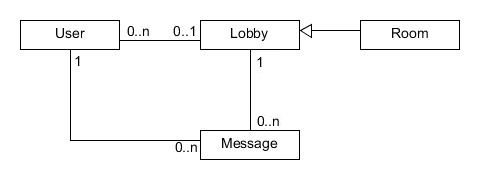
\includegraphics[width=0.7\linewidth]{img/DomainModelChatX}
\caption{Domain Model over ChatX}
\label{fig:DomainModelChatX}
\end{figure}

The domain model consists of four classes. The user class is where users are identified and if they are regular users or administrative users, a user can only be in one lobby at a time but a lobby can have multiple users. A user can also send none to many messages. The message class is used for sending messages between users, a user can have none to many messages, whilst a message can only belong to one user. The lobby is where all users start. From the lobby a user can create a room and choose which users are to be included in it, Or join a room. The room class inherits the functionality of the lobby class.